\chapter{Kinematics in One Dimension}
\section{Distance and Displacement} \index{Distance}

You are probably already familiar with the concept of \gls{distance} - you might get in your car and drive a total of 1.2 miles to school, turning right after 0.45 miles, according to your car's odometer.  Distance is a scalar that tells you how far something traveled.  The symbol d usually represents distance.

While you may have traveled a total distance of 1.2 miles from your school, you are significantly less than 1.2 miles away from home; in fact, you are approximately 0.874 miles from home, following a direct path directly from your home to the school, at an angle of $59^\circ $(not worrying that this path might take you through someone's back yard or kitchen).


  \gls{displacement} \index{Displacement} is a vector that tell you how far something is from the origin, and is independent of the path taken to get there.  The displacement vector is commonly symbolized by $\vec{d}$ though sometimes it may be written as $\vec{r}$ or $(\vec{x}-\vec{x_0})$. 

\section{Average and Instantaneous Speed and Velocity}

\gls{speed} \index{speed} is a scalar value that represents the change in distance per change in time of an object.  Speed is usually represented with the symbol $v$, without the vector sign.  You are probably already familiar with this quantity, since the speedometer on your family car measures speed.  For the purposes of physics, speed has little value because it is a scalar that tells us nothing of direction.  Much more useful is the concept called velocity.  Velocity and speed are related much like distance and displacement.  

\gls{velocity} \index{velocity} is the change in displacement of an object per unit time, and as such is a vector.  Positive velocities indicate that the object is moving forward, relative to the axis in question, and negative velocities generally mean that the object is moving backward, relative the the axis.  The average velocity of an object is given by:
\begin{mdframed}[backgroundcolor=orange!20!white]
	\begin{equation}
	\overrightarrow{v_{avg}} = \frac{\Delta\vec{d}}{\Delta t} 
		\label{eqn:velocity}
	\end{equation}
\end{mdframed}

Average velocity is useful if an object's velocity is not changing.  However, many times it is more useful to talk about instantaneous velocity.  Instantaneous velocity tells us how fast an object is moving at a given instant in time.  In order to calculate instantaneous velocity, we must allow our time interval in the above formula to become infinitesimally small.  In this case, a little calculus proves:
\begin{mdframed}[backgroundcolor=orange!20!white]
	\begin{equation}
	\vec{v} = \frac{d\vec{r}}{dt}
	\label{equation:instantaneousvelocity}
	\end{equation}
\end{mdframed}	
	
	Calculation of average velocity is rather straightforward, assuming you know both distance traveled and the time it took.  If an object is not speeding up or slowing down during a specific time interval, the instantaneous velocity at any time during this interval is equal to the average velocity.  If the object does speed up or slow down during the time interval in question, the average velocity and the instantaneous velocity at a certain time during the interval are not necessarily the same. 
	
\begin{mdframed}[backgroundcolor=blue!10!white]
		\begin{center}


		\textbf{Example \thesection.1}	
	\end{center}

\textbf{Problem: }You ride your bicycle in a straight line for a distance of 73 meters in 12.5 second.  What is your average speed?
\vspace{0.1in}

\textbf{Solution:} 
Begin by drawing a diagram:
\vspace{0.1in}

\begin{center}
	

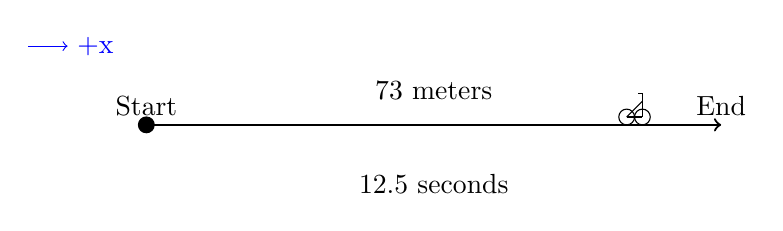
\begin{tikzpicture}
% Draw the starting point
\filldraw[black] (0,0) circle (0.1);
\node at (0,0) [above] {Start};

Draw coordiante system:
\draw[blue,->] (-1.5,1) -- (-1,1);
\node at (-1, 1) [right,blue] {+x};

% Draw the straight line representing the path


\draw[thick, ->] (0,0) -- (7.3,0);
\node at (3.65, 0.2) [above] {73 meters};

% Draw the bicycle
\draw (6.3, 0.1) circle (0.1); % Front wheel
\draw (6.1, 0.1) circle (0.1); % Back wheel
\draw (6.1, 0.1) -- (6.3, 0.1); % Frame
\draw (6.3, 0.1) -- (6.3, 0.4); % Frame
\draw (6.1, 0.1) -- (6.3, 0.3); % Frame
\draw (6.25, 0.4) -- (6.3, 0.4); % Frame

% Draw the end point
%\filldraw[black] (7.3,0) circle (0.1);
\node at (7.3,0) [above] {End};

% Draw time indication
\node at (3.65, -0.5) [below] {12.5 seconds};
\end{tikzpicture}
\end{center}

Since we have both distance and time, average speed can be easily calculated:

\begin{equation*}
 v_{avg}  = \frac{d}{t} = \frac{73m \hspace{0.05in} \hat{i}}{12.5s}  = 5.84 \frac{m}{s} \hspace{0.05in} \hat{i}
\end{equation*}

\end{mdframed}
	\vspace{0.1in}
	
\begin{mdframed}[backgroundcolor=blue!10!white]
	\begin{center}
		
		
		\textbf{Example \thesection.2}	
	\end{center}
	
	\textbf{Problem: }A bicyclist rides his bike to the east.  His position (in meters) is given by the following expression:
	\begin{equation*}
	\vec{r}(t) = (0.5 t^2 + 4t) \hat{i}
	\end{equation*}
	\begin{enumerate}[label=\alph*.]
		\item What is his average velocity from t = 0 to t = 5 seconds?
		\item What is his instantaneous velocity at t=3 seconds?
	\end{enumerate}
	\vspace{0.1in}
	\textbf{Solution:} \begin{enumerate}[label=\alph*.]
		\item The total displacement (in meters) after five seconds is given by: 
		\begin{equation*}
		\vec{d} = \vec{r}(\SI{5}{s})-\vec{r}(\SI{0}{s}) = (0.5 \times (5s)^2+4\times 5s) \hspace{0.05in} m \hspace{0.05in} \hat{i} - 0 = 32.5 \hspace{0.05in} m \hspace{0.05in} \hspace{0.05in} \hat{i}
		\end{equation*}
		Thus, the average velocity is - 
	\begin{equation*}
	\overrightarrow{v_{avg}}  = \frac{\vec{d}}{t} = \frac{32.5 m \hspace{0.05in} \hat{i}}{5s}  = \boxed{6.5 \frac{m}{s} \hspace{0.05in} \hat{i}}
	\end{equation*}
	
	
	
	\item The instantaneous velocity of an object is found using a derivative with respect to time.  Thus,
	
	\begin{equation*}
	\vec{v} = \frac{d\vec{r}}{dt} = \frac{d}{dt} (0.5 t^2 + 4t) \hat{i} = (t + 4) \hat{i} 
	\end{equation*}
	
	Evaluating this at t=3s yields:
	
	\begin{equation*}
	\vec{v} = (3 + 4) \hat{i} = 7 \frac{m}{s} \hat{i}
	\end{equation*}
	\end{enumerate}
	
\end{mdframed}

	
	
	
	

\section{Relative Motion at Constant Velocity}


\section{Acceleration}
\subsection{Average Acceleration} \index{Acceleration, Average}
Velocity is not always constant.  For instance, when you are driving through a city, there are times when you might be going 30 mph, and there are times when you might be stopped at a streetlight.  City driving requires you to speed up at some times, and slow down at other times – your velocity changes as a function of time.  Change in velocity per change in time is called \gls{acceleration}.  
Keep in mind, both speeding up and slowing down are forms of acceleration.  In the case that an object is traveling with a positive velocity, slowing down causes negative acceleration (or deceleration).
Like velocity, acceleration comes in two basic types – average and instantaneous.  To find average velocity, we calculate the change in velocity per change in time:

\begin{mdframed}[backgroundcolor=orange!20!white]
	\begin{equation}
	\overrightarrow{a_{avg}} = \frac{\Delta \vec{v}}{\Delta t} 
	\label{equation:averageacceleration}
	\end{equation}
\end{mdframed}	
Keep in mind that this can be expressed as:
\begin{mdframed}[backgroundcolor=orange!20!white]
	\begin{equation}
	\overrightarrow{a_{avg}} = \frac{\overrightarrow{v_f} - \overrightarrow {v_i}}{\Delta t}
	\label{equation:averageaccelerationalt}
	\end{equation}
\end{mdframed}	


where $v_f$ and $v_i$ are final velocity and initial velocity, respectively.  Sometimes final velocity is expressed as $v$ and initial velocity is symbolized as $v_0$. 

\subsection{Instantaneous Acceleration} \index{Acceleration, Instantaneous}

Instantaneous velocity is found by letting the time interval in question become infinitesimally small.  A little calculus proves that:
\begin{mdframed}[backgroundcolor=orange!20!white]
	\begin{equation}
	\vec{a} = \frac{d \vec{v}}{dt} 
	\end{equation}
\end{mdframed}

Combining this with equation \ref{equation:instantaneousvelocity}, we find:
\begin{mdframed}[backgroundcolor=orange!20!white]
	\begin{equation}
	\vec{a} = \frac{d^2 \vec{r}}{dt^2} 
	\end{equation}
\end{mdframed}


\begin{mdframed}[backgroundcolor=blue!10!white]
	\begin{center}
		
		
		\textbf{Example \thesection}	
	\end{center}
	\vspace{0.1in}
	
	\textbf{Problem: } A car is traveling 20 m/s in the positive x direction.  The driver sees a red light, and applies the brakes, causing the vehicle to come to a stop in 4 seconds.  What is the average acceleration caused by the brakes?
	
	\vspace{0.1in}
	
	\textbf{Solution:} First, draw the diagram:
	\vspace{0.1 in}
	\begin{center}
		

	
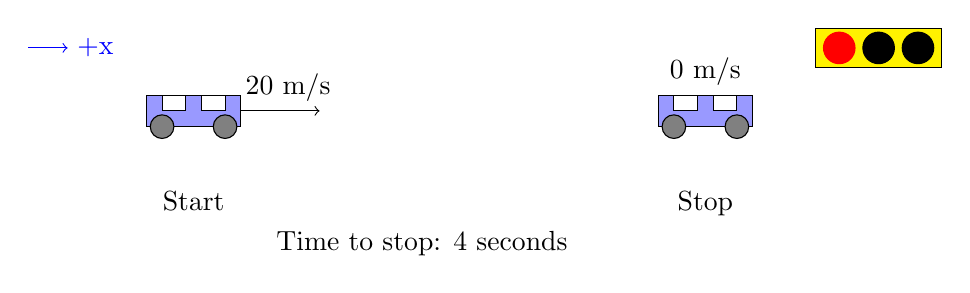
\begin{tikzpicture}
% Define car dimensions
\def\carlength{1.2} % Length of the car
\def\carheight{0.4} % Height of the car body
\def\wheelradius{0.15} % Radius of the wheels

Draw coordiante system:
\draw[blue,->] (-1.5,1) -- (-1,1);
\node at (-1, 1) [right,blue] {+x};


% Draw the initial position of the car
\draw[fill=blue!40] (0,0) rectangle (\carlength,\carheight); % Car body
\draw[fill=gray] (0.2,0) circle (\wheelradius); % Rear wheel
\draw[fill=gray] (\carlength-0.2,0) circle (\wheelradius); % Front wheel
\draw[fill=white] (0.2, \carheight-0.2) rectangle (0.5, \carheight); % Rear window
\draw[fill=white] (0.7, \carheight-0.2) rectangle (1, \carheight); % Front window
%\node at (\carlength/2, \carheight + 0.3) {20 m/s}; % Initial speed label
\node at (\carlength/2, -0.7) [below] {Start}; % Starting point label
\draw[->] (\carlength,\carheight/2) -- (\carlength+1,\carheight/2);
\node at (\carlength+0.6,\carheight/2) [above] {20 m/s};

% Draw the deceleration arrow
%\draw[thick, ->, red] (\carlength + 0.2, \carheight/2) -- (5.5, \carheight/2);
%\node at (3.5, \carheight + 0.2) [above] {Decelerating};

% Draw the red light symbol
\draw[fill=yellow] (8.5,0.75) rectangle (10.1,1.25);
\filldraw[red] (8.8, 1) circle (0.2); % Red light circle
\filldraw[black] (9.3, 1) circle (0.2); % Red light circle
\filldraw[black] (9.8, 1) circle (0.2); % Red light circle


% Draw the final position of the car
\draw[fill=blue!40] (6.5,0) rectangle (6.5+\carlength,\carheight); % Car body at final position
\draw[fill=gray] (6.7,0) circle (\wheelradius); % Rear wheel
\draw[fill=gray] (6.5+\carlength-0.2,0) circle (\wheelradius); % Front wheel
\draw[fill=white] (6.7, \carheight-0.2) rectangle (7, \carheight); % Rear window
\draw[fill=white] (7.2, \carheight-0.2) rectangle (7.5, \carheight); % Front window
\node at (6.5+\carlength/2, \carheight + 0.3) {0 m/s}; % final speed label
\node at (7.1, -0.7) [below] {Stop}; % Final point label

% Indicate time taken to stop
\node at (3.5, -1.2) [below] {Time to stop: 4 seconds}; 

\end{tikzpicture}
	\end{center}	
	
	
	 Using the definition of Average Acceleration from Equation \ref{equation:averageaccelerationalt}, we find:
	
	\begin{equation*}
			\overrightarrow{a_{avg}} = \frac{\overrightarrow{v_f} - \overrightarrow {v_i}}{\Delta t} = \frac{0 \frac{m}{s} \hat{i} - 20 \frac{m}{s} \hat{i}}{4 s}   = -5 \frac{m}{s^2} \hat{i}
	\end{equation*}
\end{mdframed}

\section{The Kinematic Equations} 
\subsection{The Kinematic Variables} \index{Kinematic Variables}
There are five variables that are often used to solve problems involving constant acceleration.  These variables are listed below:

\begin{center}
	
	
	\begin{table}[ht]\caption{\textbf{The Kinematic Variable}}% title of Table 
		\centering % used for centering table	
		\begin{tabular}{|c|c|c|}
			\hline \hline
			\textbf{Quantity} & \textbf{Variable} & \textbf{Units} \\
			\hline
			Displacement & $\vec{d}$ or $\vec{x}-\vec{x_0}$  & m \\
			\hline
			
			Initial Velocity & $\vec{v_i}$ or $\vec{v_0}$  & m/s \\
			\hline
			
			Final Velocity & $\vec{v_f}$ or $\vec{v}$  & m/s \\
			\hline
			
			Acceleration & $\vec{a}$   & $m/s^2$ \\
			\hline
			
			time & $t $  & s \\
			\hline
		\end{tabular}
		\label{table:kinematic1d}% is used to refer this table in the text
	\end{table}
\end{center}

\subsection{The Kinematic Equations}

\index{Kinematic Equations} \label{kinematicequations}
Using the definitions above, and a little calculus (or a lot of algebra) we can prove the following four equations:
\begin{mdframed}[backgroundcolor=orange!20!white]
	\begin{center}
		\textbf{The Kinematic Equations}
	\end{center}
	\begin{multicols}{2}
		\begin{equation}
		\overrightarrow{x}-\overrightarrow{x_0} = \frac{\overrightarrow{v} + \overrightarrow{v_0}}{2}  t
		\label{equation:kinematic1}
		\end{equation}
			
		\begin{equation}
		\overrightarrow{v} = \overrightarrow{v_0} + \vec{a} t
		\label{equation:kinematic2}
		\end{equation}	
			
		\begin{equation}
		\overrightarrow{x}-\overrightarrow{x_0} = \overrightarrow{v_0} t + \frac{1}{2}\vec{a}{t}^2
		\label{equation:kinematic3}
		\end{equation}
		
		\begin{equation}
		\overrightarrow{v}^2 = \overrightarrow{v_0}^2 + 2\vec{a}(\overrightarrow{x}-\overrightarrow{x_0})
		\label{equation:kinematic4}
		\end{equation}
		
		
			
		\end{multicols}
	\end{mdframed}

These equations enable you to solve the vast majority of kinematic problems.  Keep in mind that these equations should only be applied in one direction at at time – meaning that 2-dimensional and 3-dimensional problems will require you to split all the quantities into component vectors before you can solve these equations in each direction separately. It should also be noted that these equations assume constant acceleration.  If the acceleration of the object is changing, the equations are not valid.



\section{Vertical Motion and Gravity}

One of the most common types of acceleration we experience every day is the \gls{gravity}. \index{Gravity, acceleration due to}  Acceleration due to gravity is given a special symbol: $g$.  On Earth, $g \approx  \SI{9.81}{m/s^2}$.  Keep in mind that this value is only useful for calculations involving gravity that take place on the Earth's surface.  All planets, stars, and celestial bodies (in fact, all objects with any mass) have their own gravitational acceleration.  Acceleration due to gravity on the moon, for instance, is $\SI{1.62}{m/s^2}$.    

Objects undergo \gls{freefall} when the only force acting on the object is gravity.  In order to make the calculations easier, we often ignore air resistance.

Because gravity at the Earth's surface is downward, sign conventions become a little more important than previously.  If upward is positive, $g$ will have a negative sign attached to it to indicate the direction of acceleration.  


\begin{mdframed}[backgroundcolor=blue!10!white]
	\begin{center}
		
		
		\textbf{Example \thesection}	
	\end{center}
	\vspace{0.1in}
	
	\textbf{Problem: } You are standing on top of a building.  You drop a rock  from the top of the building, and let it free fall until it hits the ground, 3.2 seconds later.  
	\begin{enumerate}[label=\alph*.]
		\item What is the height of the building?
		\item An identical building is build on the moon ($g_{moon} = \SI{1.62}{m/s^2}$).  How long does it take the rock to fall in this case?
	\end{enumerate}

	\textbf{Solution:} First, draw the diagram:
	\vspace{0.1in}
	\begin{center}

	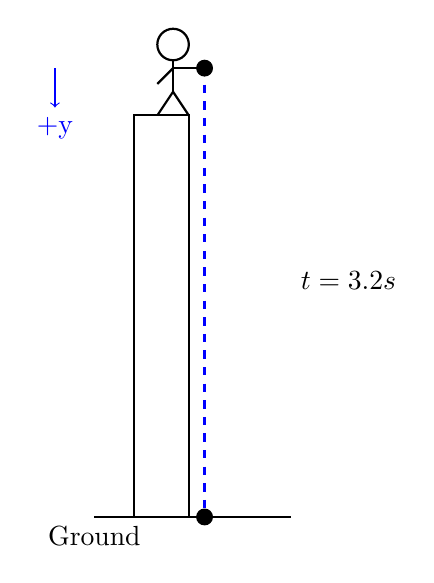
\begin{tikzpicture}


		% Draw the building
	\draw[thick] (0,0) rectangle (0.7,5.1);
%	\node at (0.5, 6.1) [above] {Top of Building}; % Label for the top of the building
	
	% Draw the person
	\draw[thick] (0.5, 6) circle (0.2); % Head
	\draw[thick] (0.5, 5.8) -- (0.5, 5.4); % Body
	\draw[thick] (0.5, 5.7) -- (0.3, 5.5); % Left arm
	\draw[thick] (0.5, 5.7) -- (0.8, 5.7); % Right arm
	\draw[thick] (0.5, 5.4) -- (0.3, 5.1); % Left leg
	\draw[thick] (0.5, 5.4) -- (0.7, 5.1); % Right leg
	
	% Draw the path of the rock
	\draw[dashed, thick, blue] (0.9, 5.7) -- (0.9, 0);
%	\node at (0.9, 3) [right] {Rock's Path}; % Label for rock's path
	
	\draw[->, blue] (-1, 5.7) -- (-1, 5.2);
	\node at (-1, 5.2) [below,blue] {+y};
	
	% Draw the rock at the top
	\filldraw[black] (0.9, 5.7) circle (0.1);
	\node at (0.9, 5.7) [right]{} ;
	
	% Draw the rock at the ground
	\filldraw[black] (0.9, 0) circle (0.1);
%	\node at (0.8, 0.2) [right] {Rock Hits Ground};
	
	% Time indication
	\node at (2, 3) [right] {$t=\SI{3.2}{s}$};
	
	% Draw the ground
	\draw[thick] (-0.5, 0) -- (2, 0);
	\node at (-0.5, 0) [below] {Ground};
	\end{tikzpicture}
	\end{center}
	
	
	\vspace{0.1 in}
	Note that we have chosen downward to be positive.  This means that gravity, displacement, and final velocity will all be positive.  Next, create a table of kinematic variables:
	
	\begin{center}
		\begin{tabular}{| r  l |}
			\hline
			$y-y_0 =$ & \\
			\hline
			$v_{0y} = $ & $\SI{0}{m/s^2}$ \\
			\hline
			$v_y = $ & \\
			\hline
			$a_y = $ & $\SI{9.81}{m/s^2}$ \\
			\hline
			$t = $ &$\SI{3.2}{s}$ \\
			\hline
		\end{tabular}
	\end{center}
	
	
	
	\begin{enumerate}[label=\alph*.]
		
		
		\item To solve for distance, we apply equation 1.5.3 in the y-direction:
		\begin{equation*}
		y-y_0 = \cancelto{0}{v_{0y}t} + \frac{1}{2}a_yt^2 = \frac{1}{2}(\SI{9.81}{m/s^2})(\SI{3.2}{s})^2 \approx \SI{50.227}{m}
		\end{equation*}
		
		\item Because we know that vi = 0 m/s, and ay = gm = 1.62 m/s2, we can let the final term drop out of equation 1.5.3 to yield:
	\end{enumerate}
\end{mdframed}




